%CS-113 S18 HW-4 Solutions
%Released: 19-March-2018
%Authors: Abdullah Zafar


\documentclass[addpoints]{exam}

% Header and footer.
\pagestyle{headandfoot}
\runningheadrule
\runningfootrule
\runningheader{CS 113 Discrete Mathematics}{Homework IV}{Spring 2018}
\runningfooter{}{Page \thepage\ of \numpages}{}
\firstpageheader{}{}{}

\boxedpoints
\printanswers
\usepackage[table]{xcolor}
\usepackage{amsfonts,graphicx,amsmath,hyperref,amssymb,amsthm,varwidth,lipsum}

\hypersetup{
    colorlinks=true,
    linkcolor=blue,
    urlcolor=cyan,
}

\title{Habib University\\CS-113 Discrete Mathematics\\Spring 2018\\HW 4 Solutions}
\date{Released: 19th March, 2018}


\begin{document}
\maketitle

\begin{questions}



\question
\begin{parts}
  \part Prove that $1 = -1 \rightarrow 2 = 1$
  
  \begin{solution}
  \begin{subparts}
  	\subpart Since the antecedent is false, the implication is true. \qed 
  			
  	\subpart Alternately, suppose \begin{align*}
			  	1 &= -1\\
			  	1 + 3 &= -1 + 3\\
			  	4 \times 0.5 &= 2 \times 0.5\\
			  	2 &= 1 \qed			  	 
  	\end{align*} 
  	\end{subparts}
  \end{solution}
  
  \part Let $a,b \in \mathbb{N}$. What's wrong with the following proof:
  \begin{align}
  a &= b\\
  a^2 &= ab\\
  a^2 - b^2 &= ab - b^2\\
  (a-b)(a+b) &= (a-b)b\\
  a+b &= b\\
  a &= 0
  \end{align}
  \begin{solution}
    Eq. 4 is being divided by $(a - b)$, which is 0 when $a=b$. 
  \end{solution}

  \part What's wrong with the following proof that shows $2^n = 1, n = \{0,1,2,...\}$, using strong induction on $n$:
  
  \textbf{Base step:} When $n=0, 2^0=1$, so the result holds.
  
  \textbf{Inductive step:} Suppose the result holds for $0\leq n \leq k$. We will show that it holds for $n=k+1$, i.e. that $2^{k+1}=1$.
  
  \begin{align*}
      2^{k+1} &= \frac{2^{2k}}{2^{k-1}}\\
      &= \frac{2^k.2^k}{2^{k-1}}\\
      &= \frac{1.1}{1}\\
      &= 1
  \end{align*}

  \begin{solution}
    The Inductive step breaks for $n=1$:
    \begin{align*}
    2^{1} &= \frac{2^{2.0}}{2^{-1}}\\
    2^{1} &= \frac{2^0.2^0}{2^{-1}}\\
    2^{1} &= \frac{1.1}{1}
    \end{align*} 
    However $2^{-1} \not = 1$ because the inductive case is undefined for $n < 0$. \qed
  \end{solution}
\end{parts}

\question Buckminster Fuller once said: ``None of the world’s problems will have a solution until the world’s individuals become thoroughly self-educated."

The world is full of problems, but which ones should you focus on? According to \href{http://8000hours.org}{80000.org}, the most urgent problems are ``not only \textbf{big}, they're also \textbf{neglected} and \textbf{solvable} - the fewer people working on a problem, the easier it is to make a big contribution. An issue can be big but comparatively well-known and crowded, like climate change, or it can be small but neglected, like land use zoning reform, and therefore also worth considering."

We present a list of the biggest, most solvable and most neglected global issues that would benefit the most from your contribution. You are encouraged to read more about how these problems measure up at \href{https://80000hours.org/articles/cause-selection/}{8000hours.org}.
\begin{center}
\begin{tabular}{ c c c}
Biosecurity & Climate change & Promoting effective altruism\\\\
Institutional decision-making & Risk from AI & Nuclear Security\\\\
Developing world health & Land use reform & Factory farming
\end{tabular}
\end{center}

You are given a set of 9 global challenges - to which you may add one more of your choice - and three order relations on them: \textbf{NB}: ``not bigger than", \textbf{NS}: ``not more solvable than" and \textbf{NN}:``not more neglected than". Using all 10 challenges and your intuition, give unique answers for each of the following. (Well-formatted, syntactically sound answers are encouraged) 

\begin{parts}
\part A poset of width 5
\part A decomposition of size 4
\part A lattice
\part A totally-ordered set
\part A well-ordered set
\end{parts}

(You may refer to the \textbf{Appendix} for a list of definitions)


  \begin{solution}
    Suppose each problem is represented with an English letter. Call this set \\
    $S = \{a, b, c, d, e, f, g, h, i, j\}.$
    
    \begin{parts}
    \part $\mathcal{P} = (S,NB)$\\
    	$NB = \{(a,b),(c,d),(e,f),(g,h),(i,j)\} \cup \{(x,x) | x \in S\}$
    	
    \part $\mathcal{P} = (S,NS)$\\
    	$NS = \{(a,b),(a,c),(a,d),(a,e),(a,f),(a,g)\} \cup \{(x,x) | x \in S\}$
    	
    \part 
    $\mathcal{P} = (S,NN)$\\
    	$NN = \{(a,b),(a,c),(a,d),(a,e),(a,f),(a,g),(a,h),(a,i)\} \\ \cup \{(a,j),(b,j),(c,j),(d,j),(e,j),(f,j),(g,j),(h,j),(i,j)\} \\ \cup \{(x,x) | x \in S\}$
    	
    \part
    $\mathcal{P} = (S,NB)$\\
    The adjacency matrix of $NB$ contains 1's at the leading diagonal, and to the right of it, and 0 otherwise.
    
    \part
    $\mathcal{P} = (S,NS)$\\
    The adjacency matrix of $NS$ contains 1's at the leading diagonal, and to the right of it, and 0 otherwise.
      	
    \end{parts}
  \end{solution}
  
\question 
A poset $(R, \preccurlyeq)$ is \textbf{well-founded} if there is no infinite decreasing sequence of elements in the poset, i.e. elements $x_1, x_2, \cdots, x_n$ such that $\cdots \prec x_n \prec \cdots  \prec x_2 \prec x_1$. A poset $(R, \preccurlyeq)$ is \textbf{dense} if for all $x \in S$ and $y \in S$ with $x \prec y$, there is an element $z \in R$ such that $x \prec z \prec y$.

Show that the set of strings of lowercase English letters with lexicographic order is neither well-founded nor dense.


  \begin{solution}
    
    Theorem: Let $ENG_l$ be the set of strings of lowercase English letters along with the lexicographic order relation $\preccurlyeq$. The poset $\mathcal{P} = (ENG_l,\preccurlyeq)$ is \textbf{neither well-founded, nor dense}.
    
    Proof: The sequence $\cdots \prec aaab \prec aab \prec ab$ is infinitely decreasing. Therefore, $\mathcal{P}$ is not well-founded. 
    
    Further, consider the two strings $a$ and $aa \in ENG_L$. There is no string $s$ such that $a \prec s \prec aa$. Therefore, $\mathcal{P}$ is not dense. \qed
     
  \end{solution}

\question
     Let $S$ and $T$ be two partial orders on a set $A$. Define a new relation $R$ on $A$ by $(x,y)\in R$ iff both $(x,y) \in S$ and $(x,y) \in T$. Prove that $R$ is a partial order on $A$.

    
      \begin{solution}
    $R$ is a partial order iff $R$ is:
    
    1) Reflexive: 
    \begin{align*}
    &\forall a \in A((a,a) \in S \wedge (a,a) \in T) \quad \quad &(S,T \text{ are reflexive})\\
    \rightarrow &\forall a \in A ((a,a) \in R) \quad \quad &(R = S \cap T)\\   
    \end{align*}
    2) Anti-symmetric:
	\begin{align*}
	&\forall a,b(((a,b) \in R \wedge (b,a) \in R)\\
	\rightarrow &((a,b) \in S \wedge (b,a) \in S) &(R \subseteq S)\\
	\rightarrow &(a = b)) &(S \text{ is anti-symmetric})\\
	\end{align*}
	3) Transitive:
	\begin{align*}
	&\forall a,b,c(((a,b) \in R \wedge (b,c) \in R)\\
	\rightarrow &((a,b) \in S \cap T \wedge (b,c) \in S \cap T) &(R = S \cap T)\\
	\rightarrow &((a,b) \in S \wedge (a,b) \in T \wedge (b,c) \in S \wedge (b,c) \in T)\\
	\rightarrow &((a,c) \in S \wedge (a,c) \in T) &(S,T \text{ are transitive})\\
	\rightarrow &((a,c) \in R)) \\
	\end{align*}
	
  \end{solution}

\question Your overly-attached girlfriend / boyfriend has concocted a cruel game to keep you around forever. The game involves piles of excuses - each pile twice as high as the last - of all the times you didn't hang out with them. Stacked in increasing order, the piles look truly endless! 

\begin{figure}[ht]
  \centering
  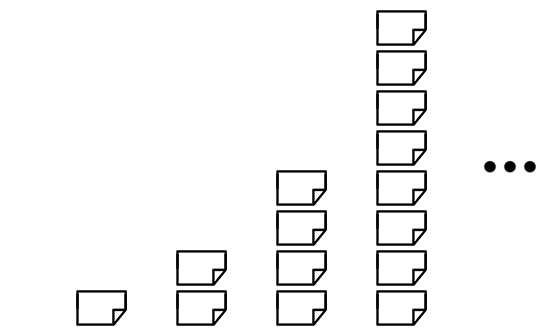
\includegraphics{excuses.png}
  \caption{That escalated quickly.}
  \label{fig:Piles of excuses}
\end{figure}

The game of \textbf{Gazillion Excuses} is a turn based 2-player game such that at each turn, a player removes a non-zero number of excuses from one of the piles. The player who removes the last excuse wins. Your partner thinks that a sufficiently large number of piles (think gazillion) would keep you playing forever. Little do they suspect that a Discrete Mathematician like yourself has formidable proof skills! Given that you are allowed to go first, \textbf{prove using induction} that you will always win the game of Gazillion Excuses. 

\begin{solution}

\textbf{Theorem}: Player 1 has a winning strategy with $k$ piles of lengths $2^0, 2^1, ..., 2^{k-1}$.

Proof: To prove our theorem, we prove the more generalized version of our setup first.
\\
\hrule
\textbf{Lemma 1}: Player 1 has a winning strategy with $N$ excuses in $k$ piles of lengths $n_1,n_2,...,n_k$, when $n_1 \oplus n_2 \oplus \cdots \oplus n_k \not = 0$.

Proof: We perform induction on the number of excuses $N$. Our proof relies on two important results which we present first.
\\
\hrule

\textbf{Lemma 2}: 

a) There exists a move that removes $x$ from $n_i$ when $n_1 \oplus n_2 \oplus \cdots \oplus n_i \oplus \cdots \oplus n_k \not = 0$, resulting in $n_1 \oplus n_2 \oplus \cdots \oplus m_i \oplus \cdots \oplus n_k = 0$, where $m_i = n_i - x$.

b) All moves that remove $x$ from $n_i$ when $n_1 \oplus n_2 \oplus \cdots \oplus n_i \oplus \cdots \oplus n_k = 0$, result in $n_1 \oplus n_2 \oplus \cdots \oplus m_i \oplus \cdots \oplus n_k \not = 0$, where $m_i = n_i - x$.

Proof: Consider binary representations of $n_1,n_2,...,n_k$ written in table form:
\begin{center}

\begin{tabular}{c | c  c  c  c}
	& $n$th bit & $n-1$th bit & $\cdots$ & $0$th bit\\
	\hline
	$n_1$ & $b_{1n}$ & $b_{1(n-1)}$ & $\cdots$ & $b_{10}$\\
	$n_2$ & $b_{2n}$ & $b_{2(n-1)}$ & $\cdots$ & $b_{20}$\\
	$\vdots$ & $\vdots$ & $\vdots$ & $\ddots$ & $\vdots$\\ 
	$n_k$ & $b_{kn}$ & $b_{k(n-1)}$ & $\cdots$ & $b_{k0}$\\
	\hline
	$\oplus$ & $b_{\oplus n}$ & $b_{\oplus(n-1)}$ & $\cdots$ & $b_{\oplus 0}$\\
	 
\end{tabular}

\end{center}

The last row is the bitwise XOR of $n_1,n_2,...,n_k$. Note that toggling any one bit $b_{ij}$ in the table toggles $b_{\oplus j}$ as well.  

a) Suppose $n_1 \oplus n_2 \oplus \cdots \oplus n_i \oplus \cdots \oplus n_k \not = 0$. Then, $\exists b \in \{b_{\oplus n},b_{\oplus (n-1)},...,b_{\oplus 0}\}(b = 1)$. Here's a strategy that ensures $\oplus n_x = 0$: Scan row $\oplus$ from left to right noting column numbers of every 1 encountered. Scan column 1 in this list from top to bottom until 1 is encountered. In this row, toggle all bits that correspond to the listed column numbers. Since toggling any one bit $b_{ij}$ in the table toggles $b_{\oplus j}$ as well, we ensure that all bits in $\oplus$ that were previously 1, are now 0. Thus $n_1 \oplus n_2 \oplus \cdots \oplus m_i \oplus \cdots \oplus n_k = 0$

b) Next, suppose that $n_1 \oplus n_2 \oplus \cdots \oplus n_i \oplus \cdots \oplus n_k = 0$. Then $\forall b \in \{b_{\oplus n},b_{\oplus (n-1)},...,b_{\oplus 0}\}(b = 0)$. Suppose $x$ excuses are removed from pile $n_i$. Then at least one bit, say $b_{ij}$, was toggled. Now $\exists b \in \{b_{\oplus n},b_{\oplus (n-1)},...,b_{\oplus 0}\}(b = 1)$. Thus, $n_1 \oplus n_2 \oplus \cdots \oplus m_i \oplus \cdots \oplus n_k \not = 0$.\\
\hrule
Now we are ready to prove \textbf{Lemma 1} via induction on $N$:

\textbf{Base case}, $N=0$:

$\oplus n_x = 0$. Player 1 loses by definition.

\textbf{Inductive step}: Suppose Lemma 1 is true for all values less than $N$. In the case of $N$ excuses, there are two cases:

1)  $n_1 \oplus n_2 \oplus \cdots \oplus n_k \not = 0$: By Lemma 2a, there exists a move for player 1 whereby $x$ excuses are removed from pile $n_i$ to give $n_1 \oplus n_2 \oplus \cdots \oplus m_i \oplus \cdots \oplus n_k = 0$. By I.H., Player 1 wins. 

2)  $n_1 \oplus n_2 \oplus \cdots \oplus n_k = 0$: By Lemma 2b, all moves by player 1 result in $n_1 \oplus n_2 \oplus \cdots \oplus m_i \oplus \cdots \oplus n_k \not = 0$. By I.H., Player 2 wins.\\

\hrule

Since our \textbf{Theorem} gives starting piles $2^0, 2^1,...,2^{k-1}$ where $2^0 \oplus 2^1 \oplus ... \oplus 2^{k-1} \not = 0$, Lemma 1 states that Player 1 will win. \qed 

 	

\end{solution}

\section{Appendix}
Let $\mathcal{P}= (P, \preccurlyeq)$,

\textbf{Chain:} A chain, $C\subseteq P$, is a subset of mutually comparable elements of $P$.\\\\
\textbf{Anti-Chain:} An anti-chain, $A \subseteq P$, is a subset of mutually incomparable elements of $P$.\\\\
\textbf{Width:} The maximum cardinality of an anti-chain of $\mathcal{P}$.\\\\
\textbf{Decomposition:} A decomposition $C$ of $\mathcal{P}$ into chains, is a family $C = \{C_1,C_2,...,C_q\}$ of disjoint chains such that their union is $P$. The size of a decomposition is the number of chains in it.


\end{questions}

\end{document}